\documentclass[11pt]{article}
\pdfinfoomitdate=1
\pdftrailerid{}
\pdfsuppressptexinfo=15
\usepackage[margin=1in]{geometry}
\usepackage[T1]{fontenc}
\usepackage{lmodern,amsmath,amssymb,amsthm,booktabs,tikz}
\usepackage[title]{appendix}
\usepackage{xurl}
\usepackage[colorlinks=true,linkcolor=blue,citecolor=blue,urlcolor=blue]{hyperref}
\hypersetup{pdftitle={The Turán density of the tight five-cycle},pdfauthor={P. Graham}}
\newtheorem{theorem}{Theorem}
\newtheorem{proposition}[theorem]{Proposition}
\newtheorem{lemma}[theorem]{Lemma}
\DeclareMathOperator{\ex}{ex}
\DeclareMathOperator{\cut}{cut}
\newcommand{\EE}{\mathbb E}
\newcommand{\ind}{\mathbf 1}
\newcommand{\Cfive}{C_5^3}
\newcommand{\fall}[2]{(#1)_{#2}}
\title{The Turán density of the tight five-cycle}
\author{P. Graham\\ \small\url{https://orcid.org/0009-0007-8493-1505}}
\date{October 27, 2026}
\begin{document}
\maketitle
\begin{abstract}
The tight five-cycle is the three-uniform hypergraph whose edges are the
five cyclically consecutive triples on five distinct vertices. We prove
that its Tur\'an density is $2\sqrt3-3$. This answers the conjecture usually
attributed to Mubayi and R\"odl, explicitly stated by Mubayi, Pikhurko and
Sudakov. Mubayi and R\"odl's recursive construction gives the lower bound.
The upper bound follows the reduction of Bodn\'ar, Le\'on, Liu and Pikhurko,
whose theorem concerns forbidding both the tight four-cycle and the tight
five-cycle, or a tight cycle of length at least seven not divisible by three. We establish the two
estimates needed for the five-cycle alone by exact rational certificates,
using weighted link inequalities to include configurations containing a
complete four-vertex hypergraph. We give the finite counting argument
that turns the certificates into these estimates and then into the density
bound. The whole proof, including this counting argument, is checked in Lean; its finite computations run as compiled code, so the check trusts Lean's compiler as well as its kernel.

This work has not yet been reviewed by experts.
The proofs, the Lean formalization and the text were produced by AI models
(from OpenAI and Anthropic), working under the author's direction.
\end{abstract}

\section{Introduction}
A three-uniform hypergraph, or $3$-graph, on $V$ is a subset of
$\binom V3$. Put
\[
 \Cfive=\bigl\{\{i,i+1,i+2\}:i\in\mathbb Z/5\mathbb Z\bigr\}.
\]
A copy in $H$ means an injective map $f:\mathbb Z/5\mathbb Z\to V$
with $\{f(i),f(i+1),f(i+2)\}\in H$ for every $i$; extra edges are allowed.
Write $f(n)=\ex(n,\Cfive)$ for the largest number of edges in a
$\Cfive$-free $3$-graph on $n$ vertices, and $\alpha=2\sqrt3-3$.

\begin{theorem}\label{thm:main}
The injective, non-induced tight five-cycle has Tur\'an density
\[
 \pi(\Cfive)=\lim_{n\to\infty}\frac{\ex(n,\Cfive)}{\binom n3}
 =2\sqrt3-3.
\]
Precisely, for every real $\varepsilon>0$ there is an integer $N\ge3$
such that for every integer $n\ge N$,
\[
 (\alpha-\varepsilon)\binom n3\le f(n)
 \le(\alpha+\varepsilon)\binom n3.
\]
\end{theorem}

Mubayi--R\"odl's Construction~1 gives the lower bound
\cite[Construction~1]{MR}\footnote{Mubayi and R\"odl credit Y.~Kohayakawa
for discussions leading to this construction \cite[\S7]{MR}.}; the equality is stated explicitly by
Mubayi, Pikhurko and Sudakov \cite[\S2.4, Conjecture~7]{MPS}.
They also record Razborov's earlier upper bound
$\pi(\Cfive)<0.4683$ \cite[\S2.4]{MPS,RazborovBound}.
The usual attribution is recorded in
Kam\v{c}ev--Letzter--Pokrovskiy \cite[Conjecture~1.1]{KLP};
their Theorem~1.3 gives the equality for all sufficiently large cycle
lengths not divisible by three.
Bodn\'ar--Le\'on--Liu--Pikhurko (BLLP) prove the equality for
$\{C_4^3,C_5^3\}$ and for $C_\ell^3$ with $\ell\ge7$ and
$3\nmid\ell$ \cite[Theorem~1.1]{BLLP}.

Falgas-Ravry and Vaughan establish the sharp bound for $3$-graphs
whose edges are the triples inducing a directed out-star in a digraph
\cite[\S3.1, Proposition~25 and Theorem~27]{FRV}.
Huang gives an analytic proof of the directed-star result
\cite[\S\S2 and~4]{Huang}. This restricted class does not include every
$\Cfive$-free $3$-graph.

The partition method and reduction are BLLP's
\cite[Propositions~3.2--3.3, Lemma~4.1 and the proof of Theorem~2.4]{BLLP}.
Here their two estimates are established for $\Cfive$ alone, with the
precise hypotheses below. The difficult step is the estimate for bad
edges minus missing triples when $K_4^3$ is allowed: BLLP identify this
obstacle in \cite[\S7]{BLLP}. The additional link inequalities below
permit exact certificates over all $\Cfive$-free six-vertex configurations.
The colored flag setup and degree and local-maximality rows follow
BLLP's supplementary calculations \cite[notebook, zero-based code cells~1 and~4]{BLLPdata}.
That notebook uses Bodn\'ar's SageMath framework, documented as
\emph{FlagAlgebraToolbox} \cite[\S\S1.2 and~2.4]{Toolbox}.
Finite sampling makes the certificate-to-graph passage explicit.
The proof depends on these computations and their Lean formalization;
Section~\ref{sec:verification} states the formal conclusion and its trust boundary.
Earlier computations for $\Cfive$ alone include Xizhi Liu's numerical
flag-algebra optimization \cite[edge-density objective and saved output]{LiuNotebook}.
The present argument supplies exact certificates and the finite estimates
needed for the unrestricted upper bound.

Ferudun's October 16, 2026 preprint \cite[Theorems~1--3 and \S5]{Ferudun}
optimizes the classical recursive construction by a logarithmic-state
algorithm and determines its quadratic term. The recursive construction
family is shared. Ferudun explicitly distinguishes this construction-side
result from an upper bound for arbitrary $\Cfive$-free hypergraphs.
The Ulam.AI UnsolvedMath record AIM-COMBINATORICS-0153 reports an exact
deficit identity, weighted stability and an optimized finite recurrence
within the same recursive family \cite{UnsolvedMath}. That summary also
leaves the unrestricted upper bound open; its underlying proof was not
read or checked here.

For the related cycle with one edge deleted, Balogh and Luo
\cite{BL} determine the density for all sufficiently long lengths
not divisible by three. Bodn\'ar, Le\'on, Liu and
Pikhurko \cite[Theorem~1.1]{BLLPminus} and, independently, Lidick\'y,
Mattes and Pfender \cite[Abstract]{LMP} determine density $1/4$.
That is a different forbidden hypergraph.

\section{Two partition estimates}
For $S\subseteq V(H)$ let $T=V(H)\setminus S$ and define
\begin{align*}
 \cut_H(S)&=|\{e\in H:|e\cap S|=2\}|,&
 \mu(H)&=\max_{S\subseteq V(H)}\cut_H(S),\\
 B_H(S)&=\{e\in H:|e\cap S|\in\{1,3\}\},&
 M_H(S)&=\{e\in\tbinom V3\setminus H:|e\cap S|=2\}.
\end{align*}
A cut is locally maximal if
$\cut_H(S\mathbin\triangle\{v\})\le\cut_H(S)$ for every $v\in V(H)$.
Thus a maximum cut is locally maximal. Write $d_H(v)$ for vertex degree,
$\beta_0=4641/10000$ and $\beta_1=464101615/10^9$.
The following are the $\Cfive$-only counterparts of BLLP's
Propositions~3.2 and~3.3; they use binomial normalization, an asymptotic
cut threshold, and coefficient one on the missing triples.

\begin{proposition}\label{prop:cut}
For every real $\varepsilon>0$ there exists an integer $N$ such that,
for every integer $n\ge N$ and every $\Cfive$-free $3$-graph $H$ on $n$
vertices, $|H|\ge\beta_0\binom n3$ implies
$\mu(H)\ge(2/5-\varepsilon)\binom n3$.
\end{proposition}

\begin{proposition}\label{prop:bad}
For every real $\xi>0$ there exist a real $\delta>0$ and an integer $N$
such that, for every integer $n\ge N$, every $\Cfive$-free $3$-graph
$H$ on $n$ vertices and every $S\subseteq V(H)$, the hypotheses
\begin{gather*}
 S\text{ is locally maximal},\qquad
 d_H(u)\le d_H(v)+\delta n^2\quad\text{for all }u,v\in V(H),\\
 \cut_H(S)\ge(2/5-\delta)\binom n3,\qquad
 |H|\ge(\beta_1-\delta)\binom n3
\end{gather*}
imply $|B_H(S)|-|M_H(S)|\le\xi n^3$.
\end{proposition}

These hypotheses are auxiliary estimates, not restrictions in
Theorem~\ref{thm:main}. In particular, the same cut of an extremal graph
will meet both estimates.

\section{Certificates and finite sampling}
The certificates use Razborov's flag algebra method \cite[\S2]{Razborov}
in the finite-sampling form described by BLLP \cite[\S3]{BLLP}. For $n\ge12$, sample an ordered
injection $(x,u,v,a,b,d)$ into $V(H)$. Write $xuv$ for the triple
$\{x,u,v\}$ in edge indicators. If a cut is present, color its
vertices by $c(z)=\ind[z\notin S]$. Let $q_K$ be the probability of its
induced six-vertex isomorphism class $K$. For any function $R$ of the
sample, let $\bar R(K)$ be its average over all $6!$ orders of $K$.
Then
\begin{equation}\label{eq:average}
 \EE R=\sum_Kq_K\bar R(K),\qquad q_K\ge0,\qquad\sum_Kq_K=1.
\end{equation}
Only $\Cfive$-free classes occur, including classes containing $K_4^3$.

\subsection*{The link inequalities}
Put $L_x(a,b)=\ind[\{x,a,b\}\in H]$ and let $K_x(a,b,c)$ indicate
that $\{x,a,b,c\}$ spans $K_4^3$. Put
\[
 C_x(a,c,d)=L_x(a,c)L_x(a,d)(1-L_x(c,d))
                  (1-\ind[\{a,c,d\}\in H]).
\]
Repeated vertices are permitted in the following sums; an edge always
has three distinct vertices.

\begin{lemma}\label{lem:link}
If $H$ is $\Cfive$-free, $x,a\in V(H)$, and $w_z\ge0$ for every
$z\in V(H)$, then
\begin{equation}\label{eq:book}
 \sum_{c,d}K_x(a,c,d)w_cw_d
 \le\sum_{c,d}C_x(a,c,d)w_cw_d.
\end{equation}
Multiplication by $w_a$ and summation over $a$ gives the corresponding
three-variable inequality. Dropping the last non-edge factor on the
right gives a further valid inequality.
\end{lemma}
\begin{proof}
For fixed $x,a$, let $F(b,c)=K_x(a,b,c)$ and
$s_c=\sum_b F(b,c)w_b$. If $F(b,c)=F(b,d)=1$, both $\{x,c,d\}$
and $\{a,c,d\}$ are absent: otherwise respectively the orders
$(c,a,b,d,x)$ and $(x,b,c,a,d)$ give a tight five-cycle.
Consequently $s_b\le m_c:=\sum_d C_x(a,c,d)w_d$ whenever $F(b,c)=1$.
Symmetry and $s_b/s_c+s_c/s_b\ge2$ give
\[
 \sum_{b,c}F(b,c)w_bw_c
 \le\sum_{b,c}F(b,c)w_bw_c\frac{s_b}{s_c}
 \le\sum_c w_cm_c.
\]
Terms of zero weight contribute zero; all denominators in a nonzero term
are positive. This proves \eqref{eq:book}.
\end{proof}

Fixing roots, restrict each free vertex by the same predicate on its
edges to the roots and its color. Applying Lemma~\ref{lem:link} with
indicator weights gives the three-variable rows, with or without the
last non-edge factor, and the two-variable rows. Nonnegative rational
weights give the weighted two-variable rows. On passing to distinct
samples the diagonal is removed, producing an error at most
$1/(n-5)$, or $W^2/(n-5)$ for two-variable weights bounded by $W$.
The diagonal is retained before this passage; it need not vanish on
$K_4^3$. Appendix~\ref{app:sampling} gives the other finite errors.

\subsection*{The cut certificate}
A selector has a specified edge or non-edge type on $(x,u,v)$ and a
rational function $p$ assigning each possible three-edge pattern of an
external vertex a probability in $[0,1]$. Given the roots, put each other
vertex in a set $U$ independently with that probability. Let $D_s$ be
the probability of the root type, and let $N_s$ be the probability of
that type together with $\{a,b,d\}\in H$ and $|\{a,b,d\}\cap U|=2$.
On a class, $\bar N_s(K)$ and $\bar D_s(K)$ denote the averages of
these same six-vertex integrands. Averaging the number of selected edges gives
\begin{equation}\label{eq:selector}
  N_s\le\frac{6D_s\mu(H)}{\fall{n-3}{3}}.
\end{equation}
Indeed, for every fixed root triple and every outcome $U$, the selected
edges avoiding the roots number at most $\cut_H(U)\le\mu(H)$; each
edge has six orders.

The rational certificate verifies, on every uncolored class,
\begin{equation}\label{eq:certificate-cut}
 \sum_s\lambda_s(\bar N_s-\tfrac25\bar D_s)
 =10^{-4}+\sum_i y_i\bar R_i+
       \sum_j\langle Q_j,A_j\rangle+h_K.
\end{equation}
Here $\lambda_s,y_i,h_K\ge0$, $\sum_s\lambda_s=1$, and every $Q_j$
is positive semidefinite. The matrices $A_j$ are products of rooted flag
indicators; $\langle Q,A\rangle=\sum_{r,t}Q_{rt}A_{rt}$.
The scalar rows are the link rows above and the two density products
$(\ind[xuv\in H]-\beta_0)\ind[abd\in H]$ and its non-edge counterpart.
All coefficients are averaged as in \eqref{eq:average}.

\begin{proof}[Proof of Proposition~\ref{prop:cut}]
Average \eqref{eq:certificate-cut} using \eqref{eq:average}.
The finite errors in Appendix~\ref{app:sampling}, weighted by the fixed
certificate coefficients, have total at most $C/(n-5)$ for all
sufficiently large $n$, where $C$ depends only on the certificate.
Thus some selector satisfies
$N_s-\frac25D_s\ge10^{-4}-C/(n-5)>0$ for all sufficiently large $n$.
Since $0\le N_s\le D_s$, its denominator is positive.
Equation~\eqref{eq:selector} now gives
$\mu(H)\ge\frac25\binom{n-3}{3}$.
Finally $\binom{n-3}{3}/\binom n3\to1$, proving the stated quantifiers.
\end{proof}

\subsection*{The bad-minus-missing certificate}
For a colored class set $t_K=(|B_K|-|M_K|)/20$. The second rational
certificate verifies, class by class,
\begin{equation}\label{eq:certificate-bad}
 t_K+\sum_j\langle Q_j,M_j(K)\rangle
       +\sum_i y_i\bar a_i(K)+\sum_j e_j\bar r_j(K)\le0.
\end{equation}
Here $Q_j$ are positive semidefinite, $y_i\ge0$, and $e_j$ may have
either sign. The rows $a_i$ express local maximality, cut density,
edge density at $\beta_1$, and the three-variable link inequality without
the last non-edge factor. The rows $r_j$ express degree differences.
Their explicit sampling functions are in Appendix~\ref{app:sampling}.
Only the matrices and multipliers are divided by the certificate's
positive integer scale; $t_K$ is unscaled.

\begin{proof}[Proof of Proposition~\ref{prop:bad}]
Each triple occurs equally often in six-sets, so
$\sum_Kq_Kt_K=(|B_H(S)|-|M_H(S)|)/\binom n3$ exactly.
For hypotheses with slack $\delta'$, averaging
\eqref{eq:certificate-bad} and using the finite errors gives
\[
 \frac{|B_H(S)|-|M_H(S)|}{\binom n3}\le A_n\delta'+K_n,
 \qquad A_n\longrightarrow A\in[0,\infty),\quad K_n\longrightarrow0.
\]
The absolute values of $e_j$ are used for degree-difference errors.
The density and cut products have lower bounds
$-\rho_n\delta'-\eta_n$, with $\rho_n\to1$, $\eta_n\to0$ as defined
in the appendix. All other errors are $O(1/n)$.
Given $\xi>0$, take $\delta=\min\{1,\xi/(A+1)\}$ and then $N$
so that $A_n\le A+1$ and $K_n\le\xi$ for every $n\ge N$.
The result follows from $2\xi\binom n3\le\xi n^3$.
\end{proof}

\section{Proof of the density theorem}
\begin{proof}[Proof of Theorem~\ref{thm:main}]
For the lower bound use Mubayi--R\"odl's construction
\cite[Construction~1]{MR}: partition into $A,B$, take every triple with
two vertices in $A$ and one in $B$, and repeat inside $B$ (Figure~\ref{fig:construction}).
A pair shared by two edges determines their construction level, so all
edges of a tight cycle would have the same level. Their three consecutive
vertices would then have a periodic part pattern with two $A$'s and one
$B$, incompatible with length five \cite[Example~1.2]{KLP}.
With $|B|/n\to r=(\sqrt3-1)/2$, the limiting density is
$3(1-r)^2r\sum_{j\ge0}r^{3j}=\alpha$; rounding and a finite-depth
approximation give $f(n)\ge(\alpha-o(1))\binom n3$.

\begin{figure}[ht]
\centering
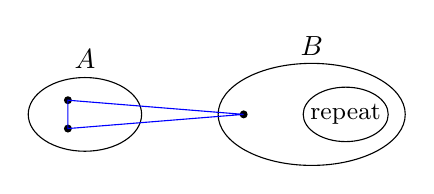
\begin{tikzpicture}[scale=0.72]
\draw (0,0) ellipse (1 and .65);\node at (0,.98) {$A$};
\draw (4,0) ellipse (1.65 and .9);\node at (4,1.2) {$B$};
\draw (4.6,0) ellipse (.75 and .48);
\node[font=\small] at (4.6,0) {repeat};
\fill (-.3,.25) circle (2pt);\fill (-.3,-.25) circle (2pt);
\fill (2.8,0) circle (2pt);
\draw[blue] (-.3,.25)--(-.3,-.25)--(2.8,0)--cycle;
\end{tikzpicture}
\caption{The recursive construction. The triangle illustrates an edge
with two vertices in $A$ and one in $B$; all such triples are included.}
\label{fig:construction}
\end{figure}

For the upper bound let $H$ attain $f(n)$.
Replacing a vertex $u$ by a clone of $v$ preserves $\Cfive$-freeness:
the collapsing map sends edges to edges, and every pair of vertices of
$\Cfive$ lies in an edge, so any cycle image is still injective.
Extremality therefore gives $d_H(v)\le d_H(u)+n$ for all $u,v$;
the possible loss is at most the codegree of $u,v$.
Choose a maximum cut $S$, which is locally maximal, and set
$s=|S|$, $m=n-s$.
Since $\alpha>\beta_0$ and $\alpha\ge\beta_1$, the lower bound,
Proposition~\ref{prop:cut}, and the degree inequality meet all the
hypotheses of Proposition~\ref{prop:bad} on this same cut for sufficiently
large $n$. For each fixed $\xi>0$ we obtain
\begin{equation}\label{eq:recursion}
 f(n)\le\binom s2m+f(m)+\xi n^3
       \le\tfrac12s^2m+f(m)+\xi n^3.
\end{equation}
Indeed, the edges consist of the cut edges, the bad edges and the edges
inside $V(H)\setminus S$; the cut edges number
$\binom s2m-|M_H(S)|$.
We may use Proposition~\ref{prop:cut} with error at most $1/5$.
For large $n$, $\binom n3\ge n^3/12$, so
$\cut_H(S)\ge n^3/60$. On the other hand
$\cut_H(S)\le s^2n/2$, which rules out $s<n/6$.
Hence $m\le5n/6$.

The scalar inequality in BLLP \cite[Fact~2.9(i)]{BLLP} is
\begin{equation}\label{eq:scalar}
 \frac{s^2m}{2}\le\frac\alpha6\bigl((s+m)^3-m^3\bigr)
 \quad(s,m\ge0).
\end{equation}
It follows from the factorization
\[
 \frac\alpha6\bigl((s+m)^3-m^3\bigr)-\frac{s^2m}{2}
 =\frac{\alpha s}{6}(s-\sqrt3m)^2\ge0.
\]

Let $D=\limsup_{n\to\infty} f(n)/\binom n3\in[0,1]$.
For every $\eta>0$ there is a constant $K_\eta$ such that
$f(m)\le(D+\eta)m^3/6+K_\eta$ for every integer $m\ge0$.
If $D>\alpha$, combine \eqref{eq:recursion}--\eqref{eq:scalar} and
$m^3\le(5/6)^3n^3$ to obtain
\[
 \frac{6f(n)}{n^3}\le\alpha+
   (D+\eta-\alpha)(5/6)^3+6\xi+\frac{6K_\eta}{n^3}
\]
for all sufficiently large $n$.
Taking a subsequence tending to the limsup and then letting $\eta,\xi$
tend to zero gives $D-\alpha\le(5/6)^3(D-\alpha)$, a contradiction.
Together with the lower bound this proves convergence and the theorem.
\end{proof}

\section{Formal verification}\label{sec:verification}
The closed Lean theorem has the following name and type, with
$\mathbb N$ and $\mathbb R$ denoting Lean's natural and real number types:
\begin{quote}\small\ttfamily\raggedright
TightCycleC5.Bridge.mubayi\_rodl\_checked :\\
Filter.Tendsto\\
\quad (fun n : $\mathbb N$ =>\\
\qquad (TightCycleC5.ex n : $\mathbb R$) / (n.choose 3 : $\mathbb R$))\\
\quad Filter.atTop (nhds (2 * Real.sqrt 3 - 3))
\end{quote}
Here \texttt{TightCycleC5.ex n} is the maximum edge count over all
finite sets $H$ of three-element subsets of \texttt{Fin n} for which
there is no injection $f:\texttt{Fin 5}\hookrightarrow\texttt{Fin n}$
with $\{f(i),f(i+1),f(i+2)\}\in H$ for every $i$; addition in
\texttt{Fin 5} is cyclic. Thus it is exactly $f(n)$ from
Theorem~\ref{thm:main}, with no induced-copy restriction or assumption
on $H$ or its partitions. Total real division defines the initial terms
for $n<3$, which do not affect the limit.

The class-by-class certificate assertions \eqref{eq:certificate-cut}
and \eqref{eq:certificate-bad}, including positivity and class coverage,
are checked in the formalization and by the accompanying exact certificate
checkers; they are not derived from a printed list of coefficients here.
The written argument proves their passage to
Propositions~\ref{prop:cut}--\ref{prop:bad} and Theorem~\ref{thm:main}.
The formal proof includes this passage and the density reduction. It
depends on 692 \texttt{native\_decide} facts, trusting Lean's compiler
and runtime as well as its kernel; it is not a kernel-only proof. These
facts check finite arithmetic, table and coefficient comparisons, and two
rational Gram identities. The class covers, arithmetic-range coverage,
all six uncolored positive-semidefinite matrices and the other 36 colored
matrices have kernel proofs.

The accompanying Lean bundle is unreleased at the time of writing.
Its checking material \cite{Checking} specifies the pinned toolchain,
all standard axioms, the exact 692-fact dependency list and reproduction
commands. The recorded full replay checked the frozen mathematical
sources; a later adapter check reused those validated dependencies and
elaborated a fresh probe of the theorem's exact type and allowed axioms.
That probe is not a second replay. The original endpoint placeholder
supplies only a type: its proof is outside the checked theorem's dependency
chain. The checking material distinguishes these executions from the
standalone Lake build, which was not exercised.

For related formalization, Jeong, Park, Hyun, Oum and Yang
\cite[Abstract]{JPHOY} formalize flag algebras for finite simple graphs.
Jeong, Park, Im, Lee and Yang combine degree-stationarity with an exact
seven-vertex certificate for the tetrahedron and formalize its bound
\cite[\S\S2.5 and~3]{Tetrahedron}.
The present development proves the finite sampling estimates for the
$3$-graphs and colored $3$-graphs used here directly.

\begin{appendices}
\section{Finite sampling estimates}\label{app:sampling}
Here are the row definitions and estimates used in the two certificate
arguments. They apply for $n\ge12$ and always to ordered injections;
$\fall n k=n(n-1)\cdots(n-k+1)$.
A flag is the induced graph, its colors when present, and its designated
ordered roots, with free vertices identified up to the specified
permutations. Its indicator vector is one-hot; a coarsening of such a
flag is also permitted.

\paragraph{Link rows.}
For roots $(x,u,v)$, let
$p(z)=(\ind[xuz\in H],\ind[xvz\in H],\ind[uvz\in H])$.
Choose a nonempty subset of its eight patterns, and optionally a set of
allowed colors. Every one of $a,b,d$ satisfies the same restriction;
a root-type indicator may also be imposed. The row is the right side
minus the left side of the three-variable version of
Lemma~\ref{lem:link}, with or without the last non-edge factor.
Its average is at least $-1/(n-5)$: the removed diagonal has at most
$(n-3)(n-4)$ terms and the conditional denominator is $\fall{n-3}3$.
For the two-variable rows fix $(x,u,v,a)$ and use a common nonnegative
weight on each free vertex determined by
\[
 (\ind[xuz\in H],\ind[xvz\in H],\ind[uvz\in H],
   \ind[auz\in H],\ind[avz\in H]).
\]
If its maximum is $W$, the diagonal weighs at most $(n-4)W^2$ and the
average is at least $-W^2/(n-5)$.

\paragraph{Positive semidefinite rows.}
For a fixed root tuple $\theta$ of a specified type, let $f_\theta$
be a one-hot flag vector and $Q$ be positive semidefinite. Put
$m_Q=\max_iQ_{ii}$. Summing all pairs of flags gives $X^TQX\ge0$,
where $X$ is the sum of their indicator vectors. Removing intersecting
free sets gives respectively the lower bounds
\[
 -\frac{m_Q}{n-5}\quad\text{(four roots)},\qquad
 -\frac{(4n-14)m_Q}{(n-4)(n-5)}\quad\text{(two roots)}.
\]
For two roots there are
$(n-2)(n-3)(4n-14)$ intersecting pairs of ordered free pairs, and
$|Q_{ij}|\le\sqrt{Q_{ii}Q_{jj}}\le m_Q$. For four roots only the
$n-4$ diagonal pairs are removed.

\paragraph{Products on disjoint triples.}
For functions $g,h$ of ordered triples, $|g|,|h|\le1$, let $\EE_3$
denote their average on a uniformly sampled ordered triple of distinct
vertices. Then
\[
 \left|\EE[g(x,u,v)h(a,b,d)]-\rho_n\EE_3g\,\EE_3h\right|
 \le\eta_n,\qquad
 \rho_n=\frac{\fall n3}{\fall{n-3}3},\quad
 \eta_n=\frac{9n^2-45n+60}{\fall{n-3}3}.
\]
This follows by removing the pairs of triples that intersect, since
$\fall n3-\fall{n-3}3=9n^2-45n+60$.
For cut rows use
$g=\ind[xuv\in H]\ind[c(x)+c(u)+c(v)=1]-2/5$;
for density rows use $g=\ind[xuv\in H]-\beta_i$.
The multiplier $h$ is a three-vertex flag indicator (the edge and
non-edge indicators in the uncolored certificate). Thus
$\EE_3g\ge-\delta'$ gives the lower bound
$-\rho_n\delta'-\eta_n$ when $h\ge0$.
The unconditional density row has lower bound $-\delta'$ exactly.
In particular, $(n-5)\eta_n\to9$; a uniform bound uses a constant
strictly larger than nine.

\paragraph{Local maximality and regularity.}
Put
\[
 \ell(x,u,v)=\ind[xuv\in H]
 (\ind[c(u)+c(v)=1]-\ind[c(u)+c(v)=0])(1-2c(x)).
\]
For every one-root flag indicator $I_F(x,a,b,d)$, local maximality gives
\[
 \EE[\ell(x,u,v)I_F(x,a,b,d)]
 \ge-\frac{6(n-3)}{(n-4)(n-5)}.
\]
For fixed $x$, the unrestricted sum of $\ell$ over ordered $(u,v)$
is $2(\cut_H(S)-\cut_H(S\triangle\{x\}))\ge0$.
The sum of $I_F$ over the free triple is nonnegative and independent
of $(u,v)$. Deleting triples meeting $\{u,v\}$ removes
$6(n-3)^2$ possibilities per fixed pair, giving the displayed bound.
For each two-root flag indicator $I_F(x,u,b,d)$, ordered degree
regularity gives
\[
 \left|\EE[(\ind[xva\in H]-\ind[uva\in H])I_F(x,u,b,d)]\right|
 \le\frac{2\delta'n^2+4n-14}{(n-4)(n-5)}.
\]
Indeed, summing over $(v,a)$ outside $\{x,u\}$ gives
$2(d_H(x)-d_H(u))$, because codegree terms cancel; at most $4n-14$
pairs meet $\{b,d\}$. Regularity is required for all ordered $x,u$,
including equality, so both signs have this bound.

\paragraph{Certificate data.}
The first certificate has nine selectors and six positive semidefinite
blocks: five with four roots and one with two. It uses the three-variable
link rows with and without the non-edge factor, the two-variable
indicator and rational-weight rows, and the two density products above.
The second has 38 blocks: three with two roots and 35 with four.
Its scalar rows comprise 80 local, eight cut, nine density and 12,750
three-variable link rows, and 120 signed regularity rows.
Each matrix entry is the joint indicator of its two flags on the
appropriate disjoint free sets; the matrix pairing includes both
ordered off-diagonal terms. In every case coefficients are rebuilt by
averaging all 720 orders of a class. With color $1$ assigned to
$V(H)\setminus S$, bad edges have color sum zero or two and missing
triples have color sum one. This explains the exact target normalization
by $\binom63=20$. These specifications, together with the rational
certificate entries, determine \eqref{eq:certificate-cut} and
\eqref{eq:certificate-bad} without any numerical optimization premise.

\end{appendices}

\begin{thebibliography}{99}

\bibitem{Checking}
P. Graham,
\emph{Checking material for The Tur\'an density of the tight five-cycle},
version 1, accompanying Lean bundle (unreleased).
The formalization guide and certificate checkers accompany the paper;
\href{../checks/FORMALIZATION.md}{formalization guide}.
Toolchain: \texttt{leanprover/lean4:v4.32.2}; Mathlib revision
\href{https://github.com/leanprover-community/mathlib4/tree/905b95818eb32af7874a58b427f50c1711a5e96c}{\texttt{905b95818eb32af7874a58b427f50c1711a5e96c}}.

\small
\bibitem{MR}
D. Mubayi and V. R\"odl,
\emph{On the Tur\'an Number of Triple Systems},
Journal of Combinatorial Theory, Series A \textbf{100} (2002), no.~1,
136--152. Author's copy, Construction~1, p.~13:
\url{https://homepages.math.uic.edu/~mubayi/papers/hypturan.pdf}.

\bibitem{MPS}
D. Mubayi, O. Pikhurko and B. Sudakov,
\emph{Hypergraph Tur\'an Problem: Some Open Questions},
October 10, 2011, \S2.4, Conjecture~7, p.~3.
\url{https://rose-kiwi.lnx.warwick.ac.uk/E/MubayiPikhurkoSudakov11aim.pdf}.

\bibitem{KLP}
N. Kam\v{c}ev, S. Letzter and A. Pokrovskiy,
\emph{The Tur\'an Density of Tight Cycles in Three-Uniform Hypergraphs},
International Mathematics Research Notices \textbf{2024} (2024), no.~6,
4804--4841. Numbering follows arXiv:2209.08134v3
(October 6, 2023; first posted September 16, 2022).
\url{https://arxiv.org/abs/2209.08134v3}.

\bibitem{BLLP}
L. Bodn\'ar, J. Le\'on, X. Liu and O. Pikhurko,
\emph{The Tur\'an density of short tight cycles},
arXiv:2506.03223v1 (first posted June 3, 2025).
All numbered references follow the versioned PDF.
\url{https://arxiv.org/abs/2506.03223v1}.

\bibitem{BLLPdata}
L. Bodn\'ar, J. Le\'on, X. Liu and O. Pikhurko,
\emph{The Tur\'an number of $\{C_5,K_4\}$}, supplementary notebook,
introduction and zero-based code cells 1--6, June 3, 2025.
\url{https://github.com/bodnalev/supplementary_files/blob/5766324d010da24a66271c0fbe38460cd377985b/no_cl/no_c5_k4.ipynb}.

\bibitem{FRV}
V. Falgas-Ravry and E. R. Vaughan,
\emph{Tur\'an H-densities for 3-graphs},
Electronic Journal of Combinatorics \textbf{19} (2012), no.~3, P40.
Numbering follows arXiv:1201.4326v1 (first posted January 20, 2012).
\url{https://arxiv.org/abs/1201.4326v1}.

\bibitem{Huang}
H. Huang,
\emph{On the maximum induced density of directed stars and related problems},
arXiv:1303.3101v2 (March 17, 2013; first posted March 13, 2013).
\url{https://arxiv.org/abs/1303.3101v2}.

\bibitem{JPHOY}
G. Jeong, S. Park, J. Hyun, S.-i. Oum and H. Yang,
\emph{Formalizing Flag Algebras in Lean},
arXiv:2607.23500v2 (October 14, 2026; first posted July 26, 2026).
\url{https://arxiv.org/abs/2607.23500v2}.

\bibitem{Toolbox}
L. Bodn\'ar,
\emph{FlagAlgebraToolbox: Flag Algebra Computations in SageMath},
arXiv:2601.06590v3 (September 12, 2026; first posted January 10, 2026).
This version documents release 0.3; the earlier supplementary notebook
\cite{BLLPdata} does not identify a release tag.
\url{https://arxiv.org/abs/2601.06590v3}.

\bibitem{Tetrahedron}
G. Jeong, S. Park, S. Im, J. Lee and H. Yang,
\emph{A New Upper Bound for the Tur\'an Density of the Tetrahedron},
arXiv:2609.27495v2 (October 2, 2026; first posted September 23, 2026).
\url{https://arxiv.org/abs/2609.27495v2}.

\bibitem{LiuNotebook}
X. Liu,
\emph{C53\_count.ipynb}, edge-density objective and saved output,
February 6, 2026, repository revision
\texttt{1b5c8b15c545ea15587f8240bd2149a29aaba857}.
\url{https://github.com/xliu2022/xliu2022.github.io/blob/1b5c8b15c545ea15587f8240bd2149a29aaba857/FlagAlgebra_Certificate/HypergraphGeneralizeTuran/script/C53_count.ipynb}.

\bibitem{Ferudun}
A. Ferudun,
\emph{An Exact Logarithmic-State Algorithm for Recursive Tight-Cycle Constructions},
version 1.0, October 16, 2026.
\url{https://doi.org/10.5281/zenodo.23421447}.

\bibitem{UnsolvedMath}
Ulam.AI, \emph{UnsolvedMath}, record AIM-COMBINATORICS-0153
(record id 20001028), research summary on recursive tight-cycle constructions.
The record metadata is dated August 14, 2026. Only the pinned dataset
record was read, not the underlying attempt or proof.
\url{https://huggingface.co/datasets/ulamai/UnsolvedMath/blob/d371ee917ac9647fbb06cd6fc529deec6f3dda82/dataset.json}.

\bibitem{BLLPminus}
L. Bodn\'ar, J. Le\'on, X. Liu and O. Pikhurko,
\emph{The Tur\'an density of the tight 5-cycle minus one edge},
arXiv:2412.21011v3 (July 9, 2025; first posted December 30, 2024).
\url{https://arxiv.org/abs/2412.21011v3}.

\bibitem{BL}
J. Balogh and H. Luo,
\emph{Tur\'an density of long tight cycle minus one hyperedge},
arXiv:2303.10530v2 (March 3, 2024; first posted March 19, 2023).
\url{https://arxiv.org/abs/2303.10530v2}.

\bibitem{LMP}
B. Lidick\'y, C. Mattes and F. Pfender,
\emph{The Hypergraph Tur\'an Densities of Tight Cycles Minus an Edge},
arXiv:2409.14257v2 (November 26, 2024; first posted September 21, 2024).
\url{https://arxiv.org/abs/2409.14257v2}.

\bibitem{Razborov}
A. A. Razborov,
\emph{Flag algebras},
Journal of Symbolic Logic \textbf{72} (2007), no.~4, 1239--1282.
\url{https://doi.org/10.2178/jsl/1203350785}.

\bibitem{RazborovBound}
A. A. Razborov,
\emph{On 3-Hypergraphs with Forbidden 4-Vertex Configurations},
2010. \url{https://doi.org/10.1137/090747476}.
The earlier upper bound is cited through the text of \cite[\S2.4]{MPS};
the original paper was not read in full.
\end{thebibliography}
\end{document}
